\chapter{Conception}
%Um am Ende der Entwicklung sichergehen zu können, dass das Programm die gewünschte Funktionalität bietet, ist es wichtig zu Beginn die Anforderungen zu definieren und das Projekt nach Abschluss damit zu evaluieren. 
%\section{Anforderungsanalyse}
%%TODO Koen: Wenn dir noch was einfällt, bitte ergänzen (und zwar direkt in den Text)
%Der Fokus dieses Projektes liegt auf die Darstellung und anschauliche Demonstration des Davis Putman Algorithmus anhand des N Damen Problems. Um dieses bestmöglich zu ermöglichen, müssen folgende Anforderungen erfüllt werden. 
%\begin{itemize}
%\item Die Größe von N für das N Damen Problem muss über eine Benutzeroberfläche veränderbar sein
%\item Bei jedem Versuch ein bestimmtes N Damen Problem zu lösen, sollen unterschiedliche Rechenwege und somit auch Lösungen entstehen. Jedoch muss aber gewährleistet sein, dass es jederzeit die Möglichkeit gibt, Ergebnisse replizierbar wiederzuzeigen. 
%\item Der Prozess zur Lösung des N Damen Problems muss einerseits auf einem Schachbrett visuell in einzelnen Schritten gezeigt und andererseits als einzelne Kalkulationsschritte wiedergegeben werden. Dabei muss zur Wahl stehen, ob der Nutzer Macro oder Micro Schritte betrachten möchte. Je nachdem welcher Schritt ausgewählt wurde, ändert sich die Größe der Zwischenschritte.
%\item Die Simualtion muss pausierbar sein.
%\end{itemize}
%Am Ende der Implementierungsphase wird das Programm anhand dieser Anforderungen gemessen und je nachdem als Erfolg oder eben als Nichterfolg deklariert. 

In order to ensure that the program offers the desired functionality at the end of the development process, it is crucial to define the requirements at the beginning and evaluate the project after completion. 
\section{Requirement Analysis}
%TODO Koen: Wenn dir noch was einfällt, bitte ergänzen (und zwar direkt in den Text)
The focus of this project is in the demonstration of the Davis Putman algorithm using the N Queens Problem. In order to achieve this in the best possible way, the following requirements must be met. 
\begin{itemize}
\item The size of N for the N Queens problem has to be modifiable via a user interface
\item With every attempt to solve a certain N Queen problem, different calculation ways and thus also solutions are to develop. However, it must be guaranteed that there is always the possibility to show replicable results. 
\item The process to solve the N Queens problem must be shown visually on a chessboard in individual steps on the one hand and reproduced as individual calculation steps on the other hand. The user must be able to choose between Macro or Micro steps. Depending on which mode was selected, the size of the intermediate steps changes.
\item The simulation must be pausable.
\end{itemize}
At the end of the implementation phase, the program is measured against these requirements and declared as successful or unsuccessful, as the case may be. 

\section{Architecture Sketch}

\section{Layout Design}
Damit die Nutzer die Animation des Davis Putman Algorithmus bestmöglich betrachten können und diesen leicht verstehen können, ist es wichtig, ein anschauliches und übersichtliches Benutzer Interface bereitzustellen. Die Interaktionen und Einstellungsmöglichkeiten müssen selbsterklärend und verständlich sein. Bereits im Vorfeld wurden deshalb verschiedene Ideen zur einem möglichen Layout gesammelt und folgendes Design wurde daraus konzepiert. 
\begin{figure}[h]
  \centering
  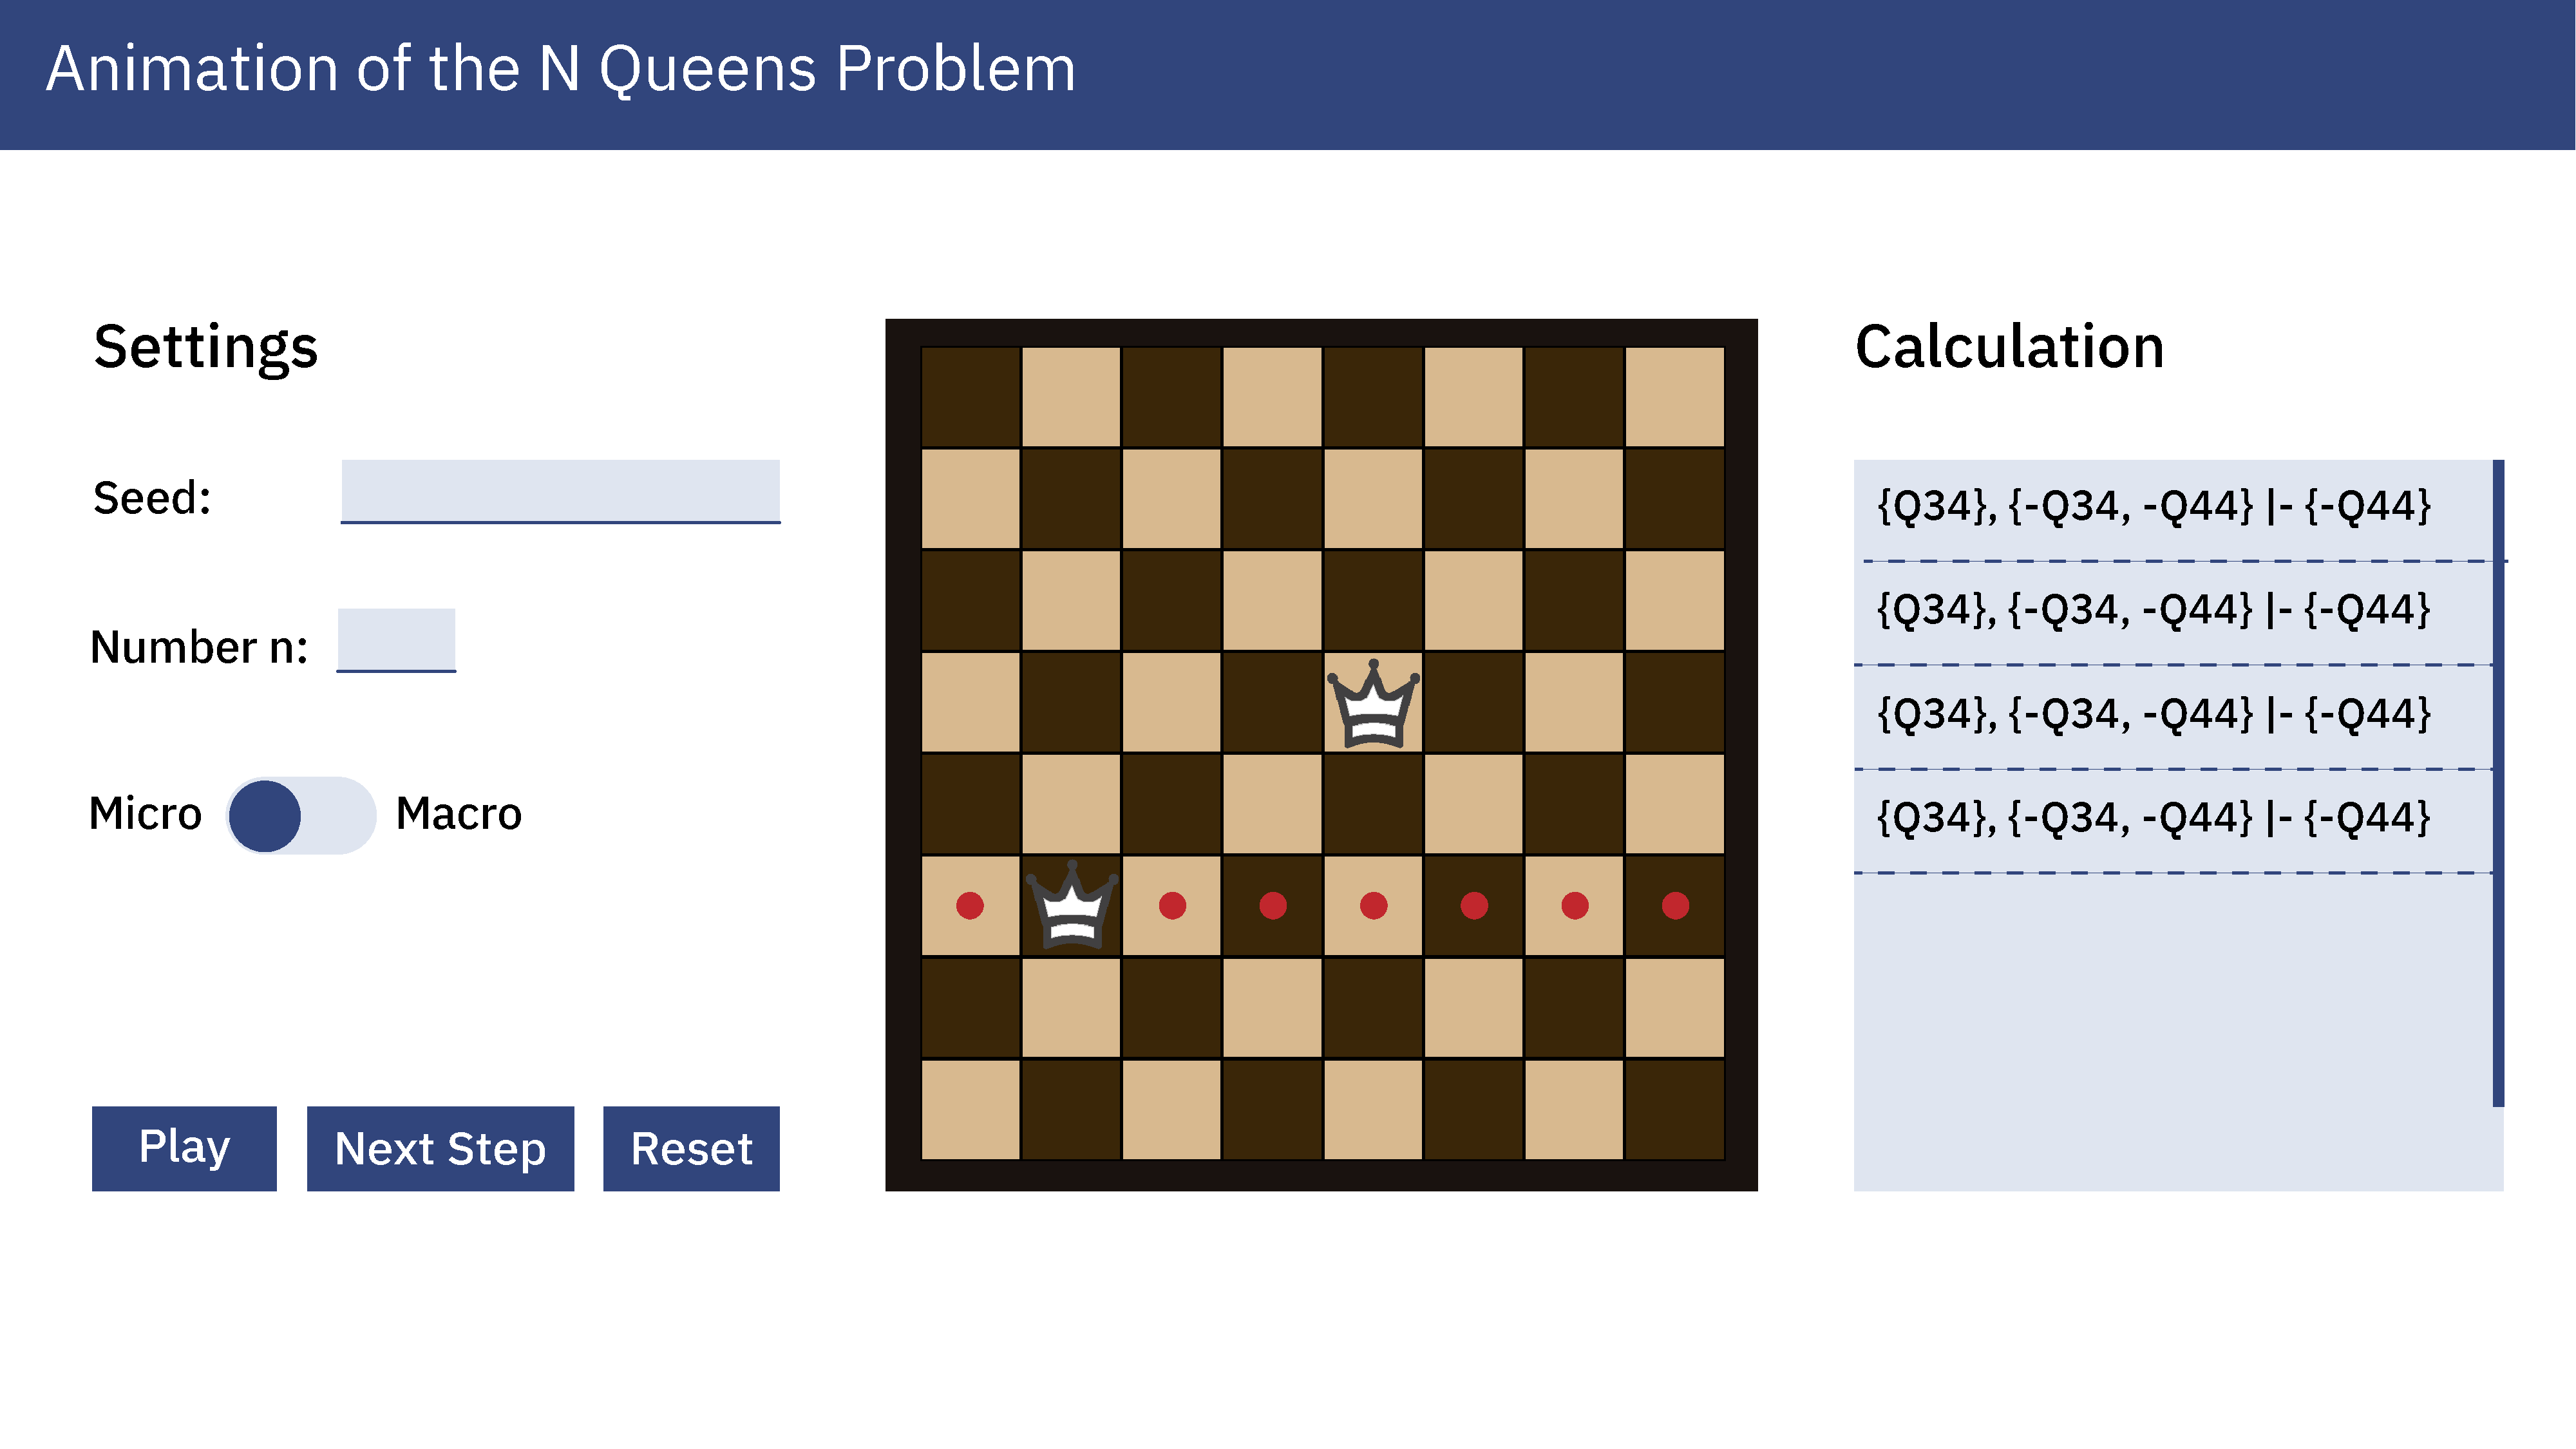
\includegraphics[width=\textwidth]{img/Design_N_Queens}
  \caption{Final Design Sketch for User Interface}
  \label{fig:design}
\end{figure}